\chapter{Feature Matching and Extraction, Camera Modelling}

The first task when we get images from various images is to extract features from these images and intersect these. So, an image of a cat from various images can be identified to be the same. Doing so will also enable us to triangulate among other applications. This chapter will also look at transformations. A feature is a piece of information which is relevant for solving the computational task related to a certain application. Features may be specific structures in the image such as points, edges or objects. Features may also be the result of a general neighborhood operation or feature detection applied to the image. The features can be classified into two main categories:

There are multiple kinds of geometry - single view, two view (\href{https://web.stanford.edu/class/cs231a/course_notes/03-epipolar-geometry.pdf}{epipolar}, projective reconstruction) where we see stereo matching (given two images, reconstruct the whole scene).

Additionally, with multiple view geometry we can stitch images together for instance - just as in panaroma.

\section{Feature Matching and Extraction}

\subsection{Detector Algorithms:} Algorithms that find interest points in an image. The interest points could be corners of an image (things which are flat and continuous surfaces may not be of interest - we need uniqueness). Now, if we use corners, they are likely unique and can be identified across images - matched in different frames. eg: Harris corner detector

\subsection{Descriptor Algorithm:} Algorithm that encodes features of the points that are identified by the detector algorithm. eg: SIFT descriptor (SIFT includes a detector as well as a descriptor)

\subsection{Image Gradients}

The image gradient along a direction, we convolve the image I with various kernels that represent the gradient along a particular direction. Hence, we are left with gradients along various directions. For instance:

\begin{equation*}
    I_x = \begin{bmatrix}-1 & 0 & 1\end{bmatrix}\cdot I
\end{equation*}

\begin{equation*}
    I_y = \begin{bmatrix}-1 \\ 0 \\ 1\end{bmatrix} \cdot I
\end{equation*}

\textbf{Gradient magnitude and direction:}

\begin{equation*}
    I_{\theta} = \tan^{-1}(\frac{I_y}{I_x})
\end{equation*}

\subsection{Harris Corner Detector} 

\begin{figure}
    \centering
    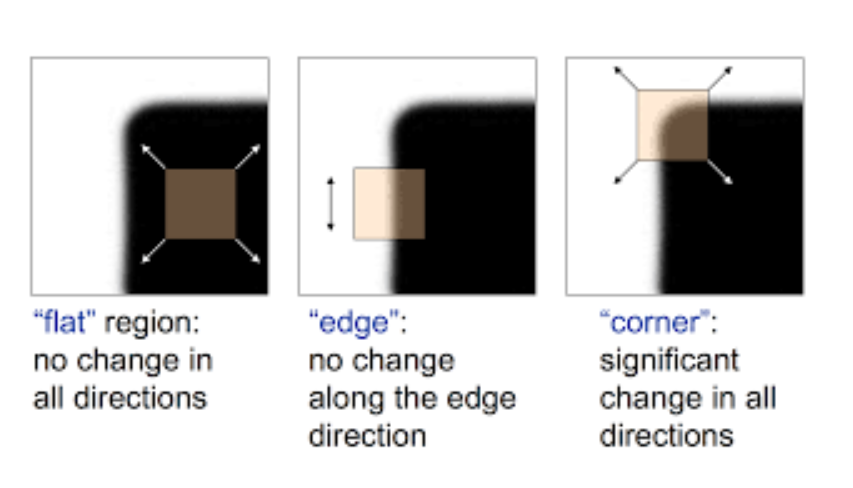
\includegraphics[width=10cm]{img/harris-corner.png}
    \caption{Harris Corner Detector}
    \label{fig:harris}
\end{figure}

The corner detector is looking for significant changes in all directions. A flat surface would have no change across any direction and a straight line feature would only change in one direction. With more directions that have gradients, we can uniquely identify it.

\subsubsection{Example of descriptor}

In a descriptor, we divide the image into several squares. For each of these squares, we will calculate the gradient and obtain the direction. Now, depending on the weight of the gradient along various directions, we will create a histogram for the gradients and choose the largest one. Now, these histograms apply only for a certain subblock of the image. If we club these histograms together, we get a feature map.

\href{https://medium.com/data-breach/introduction-to-sift-scale-invariant-feature-transform-65d7f3a72d40}{\textbf{SIFT}} is a very popular feature extraction algorithm.

\section{Frame Transformations}

The transforms that we were looking at earlier were point wise transforms. Now, we will be looking at frame wise transformations largely.

\begin{equation*}
    {}^WX=T^{World}_{Camera}{}^CX
\end{equation*}

Here, $T^{World}_{Camera}$ is the transformation that goes from world frame to camera frames. Or, it transforms from camera to world point system. Frame and point transforms are \textbf{inverse} of each other. 

\textbf{Frame perspective vs point view}.

Now when considered as frames, we multiply the transformation matrix to a point (represented relative to camera). This transformation essentially changes the basis - representing our point in a new frame. On the other hand, if we imagine the matrix as just a matrix, and consider the same basis, we can consider this to be a point transformation. But, the point transformation is in the opp direction of frame transformation.

\begin{figure}[h]
    \centering
    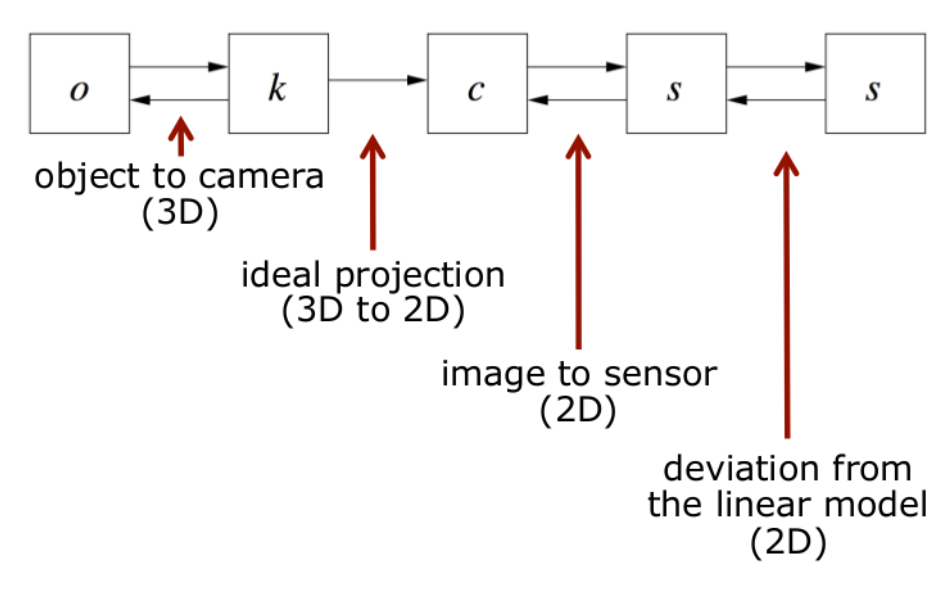
\includegraphics[width=12cm]{img/camera-pipeline.png}
    \caption{Pipeline of Transformations}
    \label{fig:pipeline}
\end{figure}

In image \ref{fig:pipeline}, first we transform from world frame to the camera frame (is invertible as inverse transformation matrix will take us from camera frame to world frame), then when we take an image, it is a projection (not invertible since we lose depth information).

Sensor will take it to an ideal space which the pinhole camera cannot take care of alone. The sensor coordinate system will hence take care of these transformations. 

\subsection{Making Transformations}

Now, we will frequently need to make transformations that rotate our camera, the object captured by the camera and so on. Since we represent everything with matrices, we also represent these transformations with matrices. How do we multiply this? There are two options: Post or pre multiplication. In general, if we post multiply, it means that the transformation was applied around the current frame. On the other hand, pre multiplying the matrix means we transform around the new frame of reference.

Look at slides \href{https://github.com/RoboticsIIITH/summer-sessions-2020/blob/master/lecture-slides/Multiple\%20View\%20Geometry/lecture-1/MVG_Session_1.pdf}{23+}. Here we have a matrix that represents the frame (by convention really) along with a camera center. Camera center - perpendicular distance between principal axis from camera center to the center of image plane.

\textbf{Something to explain slide 27 of \href{https://github.com/RoboticsIIITH/summer-sessions-2020/blob/master/lecture-slides/Multiple\%20View\%20Geometry/lecture-1/MVG_Session_1.pdf}{Rahul's slides}}

\section{Camera Modelling}

A camera's properties can be represented using a single matrix. We will use a pinhole camera here. So far, we have considered homogenous coordinates to ONLY look at points on our images. We always mentioned that these points corresponded to lines in the 3D system. Now, we will represent image points and the real world points in homogeneous coordinates:

\begin{equation*}
    \begin{bmatrix}
    X \\
    Y \\
    Z \\
    1
    \end{bmatrix}\longrightarrow \begin{bmatrix}
    fX \\
    fY \\
    z
    \end{bmatrix} = \begin{bmatrix}
    f & 0 & 0 & 0 \\\
    0 & f & 0 & 0 \\
    0 & 0 & 1 & 0 \\
    \end{bmatrix} \begin{bmatrix}
    X \\
    Y \\
    Z \\
    1
    \end{bmatrix}
\end{equation*}

where f is the focal point essentially. Look at the following image to understand the coordinates:

\begin{figure}[t]
    \centering
    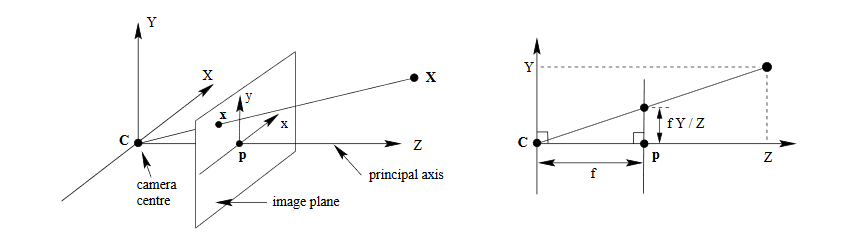
\includegraphics[width=12cm]{img/pinholecamerageometry.png}
    \caption{Pinhole Camera Geometry}
    \label{fig:pinhole-cam-geo}
\end{figure}

The matrix in this above expression can be written as $diag(f,f,1)[I|0]$, where $I$ is a $3\times3$ matrix followed by another $0$ column vector. By convention, let $X$ be the world point, and $x$ be the image point. We'll refer to the above transformation matrix as the camera projection matrix $P$. Hence,

\begin{equation}
    x = PX
\end{equation}

The above expression assumed that the origin of coordinates in the image plane is at the principal point. 

\begin{figure}
    \centering
    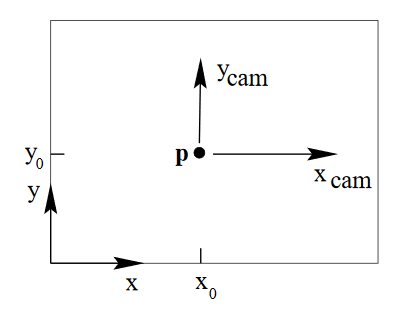
\includegraphics{img/camera-shift.png}
    \caption{Camera Shift}
    \label{fig:camera-shift}
\end{figure}

Hence, the image points will have a certain offset. Now, we will rewrite the projection matrix as follows:

\begin{equation*}
    \begin{bmatrix}
    X \\
    Y \\
    Z \\
    1
    \end{bmatrix}\longrightarrow \begin{bmatrix}
    fX \\
    fY \\
    z
    \end{bmatrix} = \begin{bmatrix}
    f & 0 & p_x & 0 \\\
    0 & f & p_y & 0 \\
    0 & 0 & 1 & 0 \\
    \end{bmatrix} \begin{bmatrix}
    X \\
    Y \\
    Z \\
    1
    \end{bmatrix}
\end{equation*}

This matrix is called the camera calibration matrix and $x = K[I|0]X_{cam}$. The camera here is located at the center of the euclidian coordinate system. 

The parameters of the matrix K are called the intrinsic parameters of the camera. Now, we can choose to change the camera orientation and position in the world coordinate system.

If we assume that the position of the camera center in the world coordinate frame is $\hat{C}$, and we rotate the camera coordinatie frame. This is a rotation and translation essentially.

Putting this together, we find that:

\begin{equation}
    x = KR[I|-\hat{C}]X
\end{equation}


